\documentclass[12pt,a4paper]{article}
\usepackage[a4paper,top=1.5cm, bottom=1.5cm, left=1.5cm, right=1.5cm]{geometry}
\usepackage[T2A]{fontenc}
\usepackage[utf8]{inputenc}
\usepackage[russian]{babel}
\usepackage{amsmath}
\usepackage{amssymb}
\usepackage{graphicx}
\usepackage{floatrow}
\usepackage{booktabs}
\usepackage{wrapfig}
\usepackage{indentfirst}
\usepackage{lipsum}
\usepackage{subcaption}
\usepackage{float}
\usepackage{derivative}
\restylefloat{table}

\newcommand{\figref}[1]{(см. рис. \ref{#1})}
\newcommand{\e}[1]{\text{$\cdot10^{#1}$}}

\title{Лабораторная работа 3.1.3\\ Измерение магнитного поля Земли}
\author{Симанкович Александр \\ Б01-104}
\date{\today}

\begin{document}
	\maketitle
	
	\section*{Цель работы}
	
	Исследовать свойства постоянных неодимовых магнитов.
	Измерить с их помощью горизонтальную и вертикальную составляющие
	индукции магнитного поля Земли и магнитное наклонение.
	
	\section*{Оборудование и приборы}
	Неодимовые магниты;
	тонкая нить для изготов­ления крутильного маятника;
	медная проволока;
	электронные весы;
	секундомер;
	измеритель магнитной индукции;
	штангенциркуль;
	брусок, линейка и штатив из немагнитных материалов;
	набор гирь и разновесов.
	
	\section*{Теоретическое введение}
	
	Магнитный момент $m$ тонкого витка площадью $S$ с током $I$:
	$$ m = IS \quad \text{(СИ)}, \qquad m = \frac{1}{c} IS \quad \text{(СГС)} .$$
	Магнитное поле точечного диполя:
	\begin{equation}
		\label{eq:magnet_dipole}
		\textbf{B}_{\text{дип}} = \frac{\mu_0}{4 \pi} \left( \frac{3(\textbf{m} \cdot \textbf{r})\textbf{r}}{r^5} - \frac{\textbf{m}}{r^3} \right) \quad (\text{СИ}), \qquad
		\textbf{B}_{\text{дип}} = \frac{3(\textbf{m} \cdot \textbf{r})\textbf{r}}{r^5} - \frac{\textbf{m}}{r^3} \quad (\text{СГС}) .
	\end{equation}
	Во внешнем магнитном поле с индукцией $\textbf{B}$ на точечный магнитный диполь $\textbf{m}$ действует механический момент сил:
	\boldmath
	$$ \mathcal{M} = [m \times B] .$$
	\unboldmath
	Потенциальная энергия диполя во внешнем магнитном поле:
	$$ W = -(\boldsymbol{m} \cdot \boldsymbol{B}) .$$
	Сила, действующая на диполь в неоднородном поле:
	$$ \boldsymbol{F} = - \nabla W = (\mathfrak{m} \cdot \nabla) \boldsymbol{B}. $$
	В частности, проекция на ось  $x$:
	$$ F_{x} = \mathfrak{m}_x \pdv{B_x}{x}
	+ \mathfrak{m}_y \pdv{B_x}{y}
	+ \mathfrak{m}_z \pdv{B_x}{z}$$
	Cила взаимодействия двух точечных диполей в случае $\mathfrak{m}_{1,2} \parallel \boldsymbol{r} $:
	$$ F_{12} = \mathfrak{m}_1 \pdv{B_2}{r} = -6 \frac{m_1 m_2}{r^4} \quad \text{(CГС)}. \qquad
	F_{12} = - 6 \frac{\mu_0}{4 \pi} \frac{m_1 m_2}{r^4} \quad \text{(СИ)}$$
	Cила взаимодействия двух точечных диполей в случае $\mathfrak{m}_{1,2} \perp \boldsymbol{r} $:
	$$ F_{12} = 3 \frac{m_1 m_2}{r^4} \quad \text{(CГС)}. \qquad
	F_{12} = 3 \frac{\mu_0}{4 \pi} \frac{m_1 m_2}{r^4} \quad \text{(СИ)}$$
	
	\subsection*{Магниты}
	
	В работе используются неодимовые магниты в форме шариков.
	Для равномерно намагниченного магнитожесткого шарика магнитное поле может быть вычислено точно. На расстояниях $r > R$ оно совпадает с полем точечного магнитного диполя \eqref{eq:magnet_dipole}. В случае $r < R$ из непрерывности нормальной компоненты индукции на поверхности шара:
	$$ \boldsymbol{B}_0 = \frac{2\mathfrak{m}}{R^3} \quad (\text{СГС}) \qquad 
	\boldsymbol{B}_0 = \frac{\mu_0 \mathfrak{m}}{2 \pi R^3} \quad (\text{СИ}). $$
	Введем \textit{намагниченность} $\boldsymbol{M} $:
	$$ \mathfrak{m} = \boldsymbol{M} V,$$
	где $V$ -- объем магнита.
	Также введем \textit{остаточную индукцию} $\boldsymbol{B}_r$:
	$$ \boldsymbol{B}_r = 4 \pi \boldsymbol{M} \quad (\text{СГС}) \qquad
	\boldsymbol{B}_r = \mu_0 \boldsymbol{M} \quad (\text{СИ}). $$
	$\boldsymbol{B}_p$ -- индукция на полюсах. Для нее выполняется:
	$$ B_p = B_0 = \frac{2}{3} B_r. $$
	
	\section*{Экспериментальная установка}
	
	\subsection*{Магнитный момент шариков}
	
	\subsubsection*{Метод А}
	
	\begin{wrapfigure}{r}{0.35\textwidth}
		\vspace{-60pt}
		\center{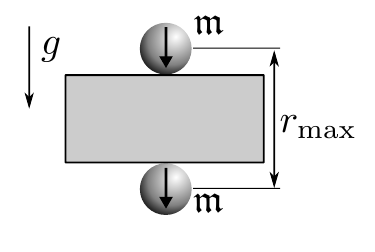
\includegraphics[width=0.7\linewidth]{res/method_A.png}}
		\caption{Определения магнитного момента шарика (Метод A).}
		\label{img:method_a}
	\end{wrapfigure}
	Величину магнитного момента m двух
	одинаковых шариков можно рассчитать, зная их массу $m$ и определив максимальное расстояние $r_{max}$, на котором они ещё удерживают друг друга в поле силы тяжести.
	$$ \mathfrak{m} = \sqrt{\frac{mgr_{max}^4}{6}} \quad (\text{СГС}) $$

	\subsubsection*{Метод Б}

	\begin{wrapfigure}{r}{0.35\textwidth}
		\vspace{-50pt}
		\center{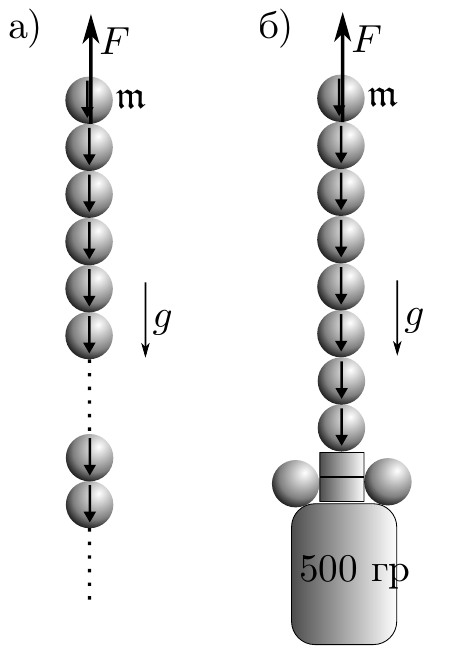
\includegraphics[width=0.5\linewidth]{res/method_B.png}}
		\caption{Определения магнитного момента шарика (Метод Б).}
		\label{img:method_b}
	\end{wrapfigure}
	Величину магнитного момен­та шариков можно определить также по си­ле их сцепления. Она определяется как сила для разрыва двух магнитных шариков. Для этого можно построить цепочку из шариков и определить, при какой длине она разорвется \figref{img:method_a}. Также нижнюю часть цепочки шаров можно заменить на массивный груз.
	
	Сила сцепления одинаковых шариков:
	$$ F_0 = \frac{3\mathfrak{m}^2}{8 R^4}. $$
	Посчитав силы взаимодействия 1-го и остальных шариков и отбросив шарики ниже 4-го получим:
	$$ F \approx 1.08 F_0. $$
	
	\subsection*{Измерение индукции магнитного поля Земли}
	
	\subsubsection*{Горизонтальная составляющая}
	\begin{wrapfigure}{R}{0.4\textwidth}
		\vspace{30pt}
		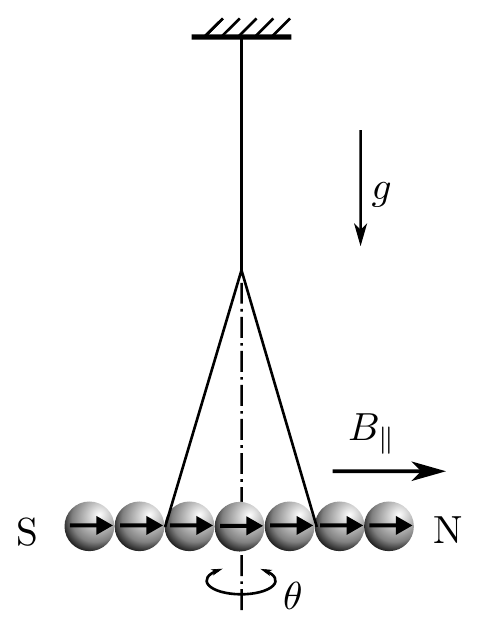
\includegraphics[width=0.8\linewidth]{res/horizontal.png}
	\end{wrapfigure}
 
	Магнитная 'стрелка' образована из $n$ сцепленных друг с другом противоположными полюсами шариков и с помощью $\Lambda$-образного подвеса подвешена в горизонтальном положении. При отклонении 'стрелки' на угол $\theta$ от равновесного положения в горизонтальной плоскости возникают крутильные колебания вокруг вертикальной оси, проходящей через середину стрелки. При малых амплитудах уравнение колебаний
	стрелки имеет вид:
	$$ J_n \dfrac{d^2 \theta}{dt^2} + \mathfrak{m}_0 B_{\parallel} \theta = 0, $$ 
	где $\mathfrak{m}_0 = n \mathfrak{m}$ -- магнитный момент стрелки, $B_{\parallel}$ -- горизонтальная составляющая магнитного поля Земли, $J_n \approx \dfrac{1}{3}n^3 m R^3$, тогда период колебаний $T = kn$, где $k = \pi \sqrt{\dfrac{md^2}{3 \mathfrak{m} B_h}}$. Измеряя зависимость $T=T(n)$, находится $B_{\parallel}$:
	$$ B_{\parallel} = \dfrac{\pi^2 m d^2}{3k^2\mathfrak{m}}. $$
	
	\subsubsection*{Вертикальная составляющая}
	
	\begin{wrapfigure}{R}{0.6\textwidth}
		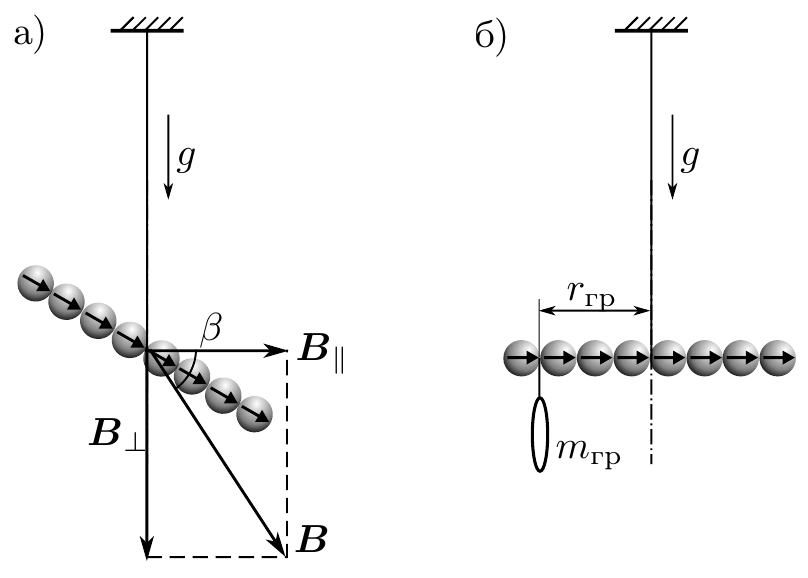
\includegraphics[width=0.8\linewidth]{res/vertical.png}
	\end{wrapfigure}
	
	Магнитная «стрелка», составленная из чётного числа
	шариков и подвешенная на тонкой нити за середину, расположится не горизонтально, а под некоторым, отличным от нуля, углом к горизонту. Это связано с тем, что вектор $\boldsymbol{B}$ индукции магнитного поля Земли в общем случае не горизонтален, а образует с горизонтом
	угол $\beta$, зависящим от географической широты $\varphi$
	места, где проводится опыт. Величина угла $\beta$
	называется магнитным наклонением.
	
	С помощью небольшого дополнительного грузика «стрелку» можно «выровнять». Момент $\mathcal{M}$ силы тяжести уравновешивающего груза пропорционален числу $n$ шариков, образующих магнитную 'стрелку':
	$$\mathcal{M}(n) = m_{\text{гр}} g r_{\text{гр}} = n \mathfrak{m} B_\perp. $$
	
	\section*{Ход работы}
	
	\section*{Вывод}
	
	
\end{document}